\section{Buildings structure}

Usually only half of the available building is used for the actual servers, while the other parts are used for cooling and energy management. 
\begin{figure}[H]
    \centering
    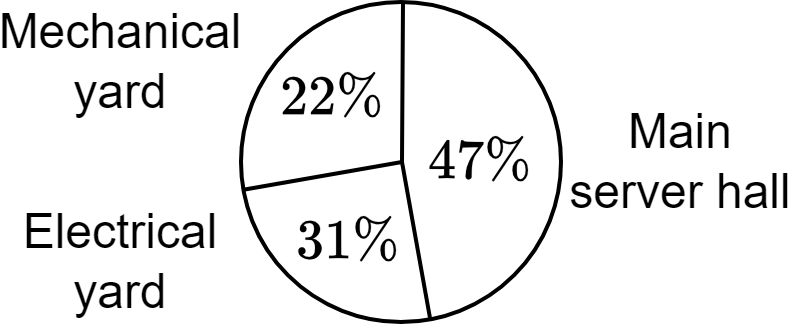
\includegraphics[width=0.5\linewidth]{images/build.png}
    \caption{Usual building usage}
\end{figure}
In addition to servers, the WSC comprises critical components associated with power delivery, cooling, and building infrastructure, all of which warrant consideration.

\subsection{Backup power generation}
To safeguard against power failure, battery systems and diesel generators are employed to back up the external power supply.
A typical Uninterruptible Power Supply (UPS) integrates three functions within a single system:
\begin{itemize}
    \item It incorporates some form of energy storage (electrical, chemical, or mechanical) to bridge the time gap between utility failure and the availability of generator power.
    \item It includes a transfer switch that selects the active power input, whether it be utility power or generator power.
    \item It conditions the incoming power feed by eliminating voltage spikes or sags, as well as harmonic distortions in the AC feed.
\end{itemize}

\subsection{Cooling systems}
IT equipment generates substantial heat, necessitating an expensive cooling system within the data center. 
This system typically includes coolers, heat exchangers, and cold water tanks.

\paragraph*{Open loop}
The most basic cooling setup is fresh air cooling, also known as air economization, which essentially involves opening windows. 
This operates as a single open-loop system.
Free cooling, or open-loop cooling, utilizes cold outside air to assist in either producing chilled water or directly cooling servers. 
While it's not entirely free in terms of cost, it incurs very low energy expenses compared to traditional chillers.

\paragraph*{Closed loop}
Closed-loop systems come in various configurations, with the air circuit on the data center floor being the most common.
The objective is to extract and expel heat from the servers, directing it to a heat exchanger. 
Cold air is directed towards the servers, where it absorbs heat and then proceeds to the heat exchanger to be cooled again for the subsequent cycle through the servers.

\paragraph*{Two-loop system}
The airflow path from the underfloor plenum, through the racks, and back to the CRAC (Computer Room Air Conditioning, a term dating back to the 1960s) delineates the primary air circuit, also known as the first loop.
The second loop, comprising the liquid supply within the CRAC units, directs from the CRAC to external heat exchangers, often positioned on the building roof. 
These heat exchangers then release the heat into the environment.

\paragraph*{Three-loop system}
A three-loop system for cooling typically involves three distinct circuits to manage the thermal environment within a data center or similar facility. Here's a brief description of each loop:
\begin{itemize}
    \item Primary air circuit: this loop involves airflow from the underfloor plenum, through the equipment racks, and back to the CRAC (Computer Room Air Conditioning) units. 
        It's responsible for regulating the temperature of the air within the data center space.
    \item Secondary liquid cooling loop: the second loop consists of a liquid coolant circulating within the CRAC units. This coolant absorbs heat from the air as it passes through the CRAC, helping to cool down the equipment and maintain optimal operating temperatures.
    \item Tertiary heat rejection loop: in this loop, the heated liquid coolant from the CRAC units is transported to external heat exchangers, typically located on the building's roof. 
        These heat exchangers release the absorbed heat into the environment, completing the cooling cycle and ensuring efficient heat dissipation from the data center.
\end{itemize}

\paragraph*{Chillers and cooling towers}
A water-cooled chiller operates similarly to a water-cooled air conditioner. 
Cooling towers are utilized to cool a water stream by evaporating a portion of it into the atmosphere. 
However, their effectiveness diminishes in very cold climates as they require supplementary mechanisms to prevent ice formation.

\paragraph*{Summary}
Each cooling topology involves trade-offs concerning complexity, efficiency, and cost:
\begin{itemize}
    \item Fresh air cooling exhibits high efficiency but is not universally applicable, necessitates the filtration of airborne particles, and may introduce intricate control challenges.
    \item Two-loop systems are straightforward to set up, relatively cost-effective to build, and provide isolation from external contaminants. 
        However, they generally exhibit lower operational efficiency.
    \item Three-loop systems are the most costly to establish and involve moderately complex controls. 
        However, they offer protection against contaminants and boast good efficiency.
\end{itemize}

\paragraph*{Liquid cooling}
An in-rack cooler integrates an air-to-water heat exchanger at the rear of a rack, allowing hot air emitted by the servers to pass over coils cooled by water. 
This setup significantly shortens the distance between server exhaust and the input of the CRAC (Computer Room Air Conditioning) unit.

In-row cooling functions similarly to in-rack cooling, but instead of having the cooling coils within the rack, they are positioned adjacent to the rack.

Direct cooling of server components is achievable through cold plates, which are essentially local liquid-cooled heat sinks. 
However, it's impractical to cool all compute components using cold plates. 
Typically, components with the highest power dissipation are targeted for liquid cooling, while other components rely on air cooling. 
The liquid circulating through the heat sinks carries the heat to a liquid-to-air or liquid-to-liquid heat exchanger, which can be situated near the tray or rack, or be integrated into the data center infrastructure, such as a cooling tower.

\paragraph*{Container-based datacenters}
Container-based data centers represent a further advancement from in-row cooling by housing server racks within a container, typically ranging from six to twelve meters in length. 
These containers integrate heat exchange and power distribution systems directly into the container structure.

\subsection{Datacenter power consumption}
Data center power consumption has become a critical issue due to its potential to reach several megawatts (MWs). 
Cooling requirements typically consume around half of the energy needed by the IT equipment, including servers, network infrastructure, and disks.
Moreover, the energy transformation processes within data centers often result in significant energy wastage.

In terms of global impact, data centers account for approximately 3\% of the world's electricity supply, exceeding the annual electricity consumption of countries like the UK, which stands at 300 terawatt-hours (TWh). 
This substantial power consumption contributes to about 2\% of total greenhouse gas emissions, comparable to the emissions produced by worldwide air traffic before the pandemic.

The carbon dioxide (CO2) emissions from data centers are substantial, equivalent to the emissions of entire countries such as the Netherlands or Argentina. 
This highlights the urgent need for energy-efficient solutions and sustainable practices within the data center industry to mitigate its environmental impact.

The power consumption of data centers poses a significant challenge, as it can scale up to multiple megawatts (MWs). 
Typically, cooling operations account for approximately half of the total energy consumption, encompassing the energy demand of IT equipment such as servers, network infrastructure, and disks. 
Additionally, the energy transformation processes within data centers result in substantial wastage, further contributing to the overall energy consumption.

\paragraph*{Power usage effectiveness}
Power Usage Effectiveness (PUE) represents the ratio of the total energy consumed by a data center facility to the energy supplied to the computing equipment, expressed as:
\[\text{PUE}=\dfrac{\text{Total Facility Power}}{\text{IT Equipment Power}}\]
Here, total facility power encompasses the energy consumption of IT systems, including servers, network devices, and storage units, along with other equipment such as cooling systems, Uninterruptible Power Supplies (UPS), switch gear, generators, lighting, and fans.
Data Center Infrastructure Efficiency (DCiE) is the reciprocal of Power Usage Effectiveness (PUE).

\subsection{Taxonomy}
Data center availability is categorized into four distinct tier levels, each with its own set of requirements.
\begin{table}[H]
    \centering
    \begin{tabular}{|c|l|}
    \hline
    Tier level & \multicolumn{1}{c|}{Requirements} \\ \hline
    1          & \makecell[l]{No redundancy \\ 99.671\% uptime per year \\ Maximum of 28.8 hours of downtime per year }                                 \\\hline
    2          & \makecell[l]{Some cooling and power redundancies \\ 99.741\% uptime per year \\ No more than 22 hours of downtime per year}    \\\hline
    3          & \makecell[l]{$N+1$ fault tolerance \\ 99.982\% uptime \\ Less than 1.6 hours of downtime per year} \\\hline
    4          & \makecell[l]{$2N$ or $2N+1$ fault tolerance \\ No single points of failure \\ 99.995\% uptime per year \\ Less than 26.3 minutes of downtime per year}                                 \\ \hline
    \end{tabular}
\end{table}
